%!TEX ROOT=../dissertation.tex

\chapter{Natural Language Inference}
\label{chap:nli}

In chapter~\ref{chap:pipeline}, we have discussed the methods chosen by the \textsf{FCheck} team to retrieve a set of evidence relevant to the given claim. In the following chapter, we will proceed to show how to use these sets of evidence to infer whether the claim is provable or refutable.

This task is widely known as the \textit{Natural Language Inference} (NLI), previously known as the \textit{Recognizing Textual Entailment} (RTE). Whereas the RTE classification is bipartite (\textit{entailed}, \textit{no entailment}), the standard NLI classification is tripartite (\textit{entailed}, \textit{negation entailed}, \textit{no entailment})~\cite{overview}.

\section{Task definition}
\label{sec:task}
Given a textual claim $c_i$ and its set of evidence $E_{c_i}$ from the knowledge base, give a veracity label

$$h(c_i,E_{c_i}) = y$$

\noindent where $y\in\{\texttt{SUPPORTS},\texttt{REFUTES},\texttt{NOT ENOUGH INFO}\}$

\vspace{.3em}
For a practical instance, given a blinded datapoint formatted as in~\ref{list:fcheck-nli}, give the corresponding \texttt{label} given the \texttt{claim} and a \texttt{context}.

\section{Related work}
\label{sec:nlicorp}
We have examined the following NLI datasets in English, and their respective state-of-the-art classifiers, largerly based on transformer models resemblant to \textsf{BERT}~\cite{devlin2019bert}
\begin{itemize}
    \item {\techbf Stanford NLI Corpus} ({\techbf SNLI})~\cite{snli:emnlp2015}: \"{A large annotated corpus for learning natural language inference} -- a long-term standard benchmark for the task of natural language inference. Corpus of \char`~570,000 human-written English sentence pairs manually labeled for balanced classification as \texttt{entailment}, \texttt{contradiction} or \texttt{neutral}.
    
    The state-of-the-art classifier as of May 2021 is \textsf{EFL}~\cite{wang2021entailment}, which reaches 93.1\% accuracy on the testing set. It uses a few-shot learning of \textsf{RoBERTa}~\cite{roberta} on the specific NLI classes.
    
    \item {\techbf Multi-Genre Natural Language Inference} ({\techbf MultiNLI})~\cite{multinli} was collected for the \textsf{RepEval} shared task. It is  modeled after \textsf{SNLI} and distributed in the same format. It contains \char`~433,000 sentence pairs and covers various genres of spoken and written English, such as \textsc{Fiction} extracted from project \textsf{Gutenberg}\footnote{\url{https://gutenberg.org}}, \textsc{Travel} from \textsf{Berlitz} travel guides, etc\dots
    
    As of May 2021, The highest accuracy (92.2\% in \textsc{Matched}, 91.7\% in \textsc{Mismatched}) was reached by \textsf{Google}'s \textsf{T5-11B}\footnote{Stands for a \textbf{T}ext-\textbf{t}o-\textbf{T}ext \textbf{T}ransfer \textbf{T}ransformer with \textbf{11 B}illions of parameters.}~\cite{t5-11b} through \textit{transfer learning}, i. e. fine-tuning a large model pretrained on a data-rich task to the specific downstream task of NLI.
    
    \item {\techbf Adversarial NLI} ({\techbf ANLI})~\cite{anli} - human-and-model-in-the-loop dataset, consisting of three rounds of increasing complexity and difficulty (\textsf{A1}, \textsf{A2}, \textsf{A3}), that include explanations provided by annotators. The total size of all sets is about 170K sentence pairs.
    
    The state-of-the-art solver \textsf{InfoBERT}~\cite{infobert} applies a further adversarial training to the \textsf{RoBERTa} model to achieve 75\% accuracy on the \textsf{A1} test set and 58.3\% overall, using all the samples of \textsf{A1}, \textsf{A2}, \textsf{A3} test sets combined.
    \item {\techbf FEVER for NLI} is a simple conversion of the \textsf{FEVER} dataset from its original format to the $(query,context)$ pairs, made as a byproduct of the UNC classifier~\cite{nie2019combining} from the \textsf{FEVER} shared task.
    
    This specific classifier was taught using NSMN\footnote{Neural Semantic Matching Network} augmented by a \"{relatedness} score and ontological knowledge from \textsf{WordNet}, and achieved  68.16\% label accuracy. 
\end{itemize}

\subsection{Slavonic Language Models}
As nearly every solution examined in the Section~\ref{sec:nlicorp} relies on the transfer learning, fine-tuning a large Transformer (\ref{sec:transformers}) language model to learn the predictions on a \textit{down-stream} task, let this be the strategy we employ for the preliminary entailment experiments as well.

First of all, let us examine the models that may already \"{speak} Czech: 
\begin{itemize} 
    \item {\techbf{Multilingual BERT}} ({\techbf mBERT}) -- is, basically, a variation of \textsf{Google}'s famed \textsf{BERT}$_\textsf{BASE}$ model~\cite{devlin2019bert} for multiple languages, trained on the \textit{Masked Language Modeling} (\textit{MLM}) and \textit{Next Sentence Prediction} (\textit{NSP}) tasks using 104 localizations of \textsf{Wikipedia}. In our team, it has already been used for the \textit{knowledge scope} computations (\ref{sec:knowledge-scopes}), as well as for the Document Retrieval task by~\cite{rypar,michal} (\ref{tab:dr}) towards encouraging results
    
    \item {\techbf{SlavicBERT}}~\cite{slavicbert} -- similar to \textsf{mBERT}, trained on joint Bulgarian, Czech, Polish and Russian corpora
   
   \item {\techbf{HerBERT Ullrich}} -- haha, nothing here. Just testing your \textit{attention} (\ref{sec:transformers})\footnote{\textit{Ba dum tss.}}
   \item {\techbf XLM-RoBERTa}~\cite{xlm-roberta} is the crosslingual version of \textsf{RoBERTa}, trained solely on the \textit{MLM} task on a corpus significantly larger than of \textsf{Wikipedia} -- the cleaned \textsf{CommonCrawl} data it is trained on comes at 2.5TB of storage-size. As of May 2021, the \textsf{RoBERTa} derivates achieve thestate-of-the-art performance in many NLI benchmarks\footnote{See at \url{https://paperswithcode.com/task/natural-language-inference/latest}}
    \item {\techbf{CZERT}}~\cite{czert} is a recent arrival to the \textsf{BERT} family -- a couple of monolingual Czech models that are trained using 340K sentences from the Czech \textsf{Wikipedia}, \textsf{Czech National Corpus} and crawled Czech news. The models are based on \textsf{BERT} and \textsf{ALBERT}~\cite{albert} and are trained with random initialization on the \textit{MLM}+\textit{NSP} and \textit{MLM}+\textit{Sentence Order Prediction} tasks, respectively.
\end{itemize}
\section{Modified ČTK dataset}
\label{sec:modified-ctk}
On top of the \textsf{ČTK} dataset~(Section \ref{sec:dataset-latest}), we propose the following simple methods of augmentation for the NLI task, using the auxiliary data collected in Chapter~\ref{chap:collection}.

To emulate a set of evidence for the \texttt{NOT ENOUGH INFO} annotations in task~\ref{sec:task}, one can simply sample paragraphs from the knowledge scope of this claim. We propose to sample multiple different evidence sets for a single \texttt{NEI} claim in order to balance the dataset.

In~\ref{sub:conditional}, we have introduced the concept of \textit{conditional labeling}. In terms of natural language inference, the labels with nonempty \texttt{condition} can be included twice:

\begin{enumerate}
    \item As \texttt{NOT ENOUGH INFO} annotations
    \item As \texttt{SUPPORTS} or \texttt{REFUTES} annotations, if we consider larger evidence sets, augmented with the knowledge listed in \texttt{condition}
\end{enumerate}

This behaviours have been added to our dataset export \textsf{API} (\ref{sec:export}) using the \textsf{HTTP GET} activation parameters \texttt{simulateNei=1} and \texttt{condition=double}, respectively.

\section{NLI Experiments}

In the following section, we will conclude a set of preliminary Natural Language Inference experiments, largely relying on the \textsf{AIC FactCheck}'s internal set of modules for model training and evaluation by~\cite{honzagit}, that has shown promising preliminary results after the first wave of annotations. 

The \textsf{BERT}-like models are handled with ease using the \textsf{Huggingface} \texttt{transformers}~\cite{huggingface} and the \textsf{sBERT} \texttt{sentence\_transformers} \cite{sentence-transformers} libraries. We would like to thank the authors of all the aforementioned software for making it easy to obtain relevant results without having to delve too deep into the underlying compatibility challenges.

\subsection{Data Consistency Remarks}
As the experiments from this chapter were to be run simultaneously with the dataset collection and evaluation from the Chapters~\ref{chap:ctk}  and~\ref{chap:dataset}, naturally, we have run into a \textit{race condition}. That is, at a certain point we had to fix a single legacy dataset version to be used for all further runs of our experiments and to proceed with the production dataset refinement in separation from the NLI application. 

The dataset we fixed for this task is the \textsf{ČTK v2 CSV} (\ref{item:ctk-csv}) exported in early May 2021, that does not yet include all the refinements described in Chapter~\ref{chap:dataset}. However, it features all the datapoints from the first three waves, similarly to \textsf{ČTK v2.1}. For the completeness, we attach the \textsf{JSONL} reprint of the data in our dataset cloud storage\footnote{\url{http://bertik.net/ctk}}, even though in practice it is being generated on-demand from the \textsf{CSV db} dump using a fixed\textit{ seed of randomness}. 

As we will be using the \textit{stratified} split of our dataset, de facto disabling the \textit{accuracy} metric, we will be comparing our models based on their the $F$-score, which is a standard benchmark for the NLI task~\cite{poliak}.

\subsection{Experiments on Sentence\_transformers Models}
\label{sec:expts}
Using a set of ad--hoc \textsf{Jupyter} notebooks\footnote{\url{https://gitlab.fel.cvut.cz/factchecking/nli}} powered by the \textsf{sentence\_transformers} and the shared codebase of the \textsf{AIC/FactCheck} team, we have downloaded the pretrained \textsf{SlavicBERT} and \textsf{mBERT} models in their \textit{cased} defaults, provided by the \textsf{DeepPavlov}~\cite{deeppavlov}. Furthermore, we have acquired an \textsf{XLM-RoBERTa} model, fine-tuned on an NLI-related \textit{SQuAD2}~\cite{squad} \textit{down-stream task}. This model was provided by \textsf{deepset}~\cite{deepset}.



Starting from these three base models, we have initiated a series of model training tasks on the \textsf{RCI Cluster}, varying in the batch size and the overall number of epochs. The latter was typically not of an overwhelming significance, as, given the relatively small \textsf{train} split of the \textsf{ČTK} dataset, models soon started to overfit -- see Figure~\ref{tab:overfitting}. In such cases, we kept the \textsf{dev}-optimal model, tossing the later epochs.

%%%%

\begin{table}[H]
\begin{ctucolortab}
\begin{tabular}{|c|c|c|}
\hline
\textbf{epoch} & \textbf{\textsf{train} acc. }   &\textbf{ \textsf{dev} acc.}    \\
\hline
0.     & 0.80 & 0.77  \\
1.     & 0.93 & \textbf{0.87}  \\
2.     & 0.96 & 0.81  \\
3.     & 0.98 & 0.85 \\
4.     & 0.98 & 0.84 \\
 \vdots      & \vdots   &  \vdots \\
100.   & \textbf{1.00}  & 0.81 \\  
\hline
\end{tabular}
\end{ctucolortab}
\caption{The progress of \textsf{XLM-RoBERTa@SQuAD2\_bs4} in the \textsf{train} and \textsf{dev} accuracies during 100 epochs of training on the \textsf{ČTK} dataset}
    \label{tab:overfitting}
\end{table} % Overfit

Despite that, we have set a strong baseline for the future NLI experiments on the \textsf{ČTK} datasets with our \textsf{XLM-RoBERTa} model scoring an $F$-value of \textbf{0.86}. For reference, the \cite{fever} baseline scored 80.82\% \textit{accuracy} in a similar setting (\textit{NearestP} -- nearest page for a \textsf{NEI} context) on \textsf{Wikipedia}, using a Decomposable Attention model.

\begin{table}[H]
    \centering
    \makebox[\textwidth][c]{\begin{ctucolortab}
    \begin{tabular}{|lr|rr|rr|}
    \hline
    \textbf{\textsf{ČTK v2 CSV} split:}&&\multicolumn{2}{c|}{\textsf{test}}&\multicolumn{2}{c|}{\textsf{dev}}\\
    \hline
    \textbf{model}&\footnotesize{$|batch|$}& \textbf{\footnotesize{micro-}$F_1$}&\textbf{\footnotesize{macro-}$F_1$} &\textbf{\footnotesize{micro-}$F_1$}&\textbf{\footnotesize{macro-}$F_1$}\\
    \hline
        \textsf{SlavicBERT} &2 &\textit{0.743}&0.700&0.771&0.735\\
        \textsf{SlavicBERT} &5 &\textit{0.741}&0.702&0.782&0.757\\
        \textsf{mBERT} &3 &\textit{0.727}&0.686&0.710&0.667\\
        \textsf{mBERT} &10 &\textit{0.743}&0.717&0.742&0.721\\
        \textsf{XLM-RoBERTa @ SQuAD2} &2 &\textit{0.807}&0.769&0.842&0.815\\
        \textbf{\textsf{XLM-RoBERTa @ SQuAD2}} &\textbf{4} &\textbf{\textit{0.855}}&\textbf{0.840}&\textbf{0.866}&\textbf{0.849}\\
        \textsf{XLM-RoBERTa @ SQuAD2} &7 &\textit{0.835}&0.819&0.851&0.838\\
        \hline
    \end{tabular}
    \end{ctucolortab}}
    \caption[$F$-score comparison of our \textsf{BERT}-like NLI models]{$F$-score (\textbf{micro-$F_1$}) comparison of our \textsf{BERT}-like models for the \textit{NLI} task on the {\techbf ČTK} data, experimenting with different training \textit{batch sizes}. \textit{Coursive} decisive, \textbf{bold} best.}
    \label{tab:nli}
\end{table} % f1
%%%

Furthermore, we render the confusion matrices for two of our strongest models -- the \textsf{XLM-RoBERTa} and the \textsf{SlavicBERT}, to see the distribution of their \textsf{test}-set \textit{(mis-)classifications} -- we see that the main disadvantage of \textsf{SlavicBERT} compared to the stronger \textsf{XLM-RoBERTa} is the understanding of the \texttt{REFUTES} annotations.
%--- FIG: UTF forms
\begin{figure}[H]
\vspace{2em}
\makebox[\textwidth][c]{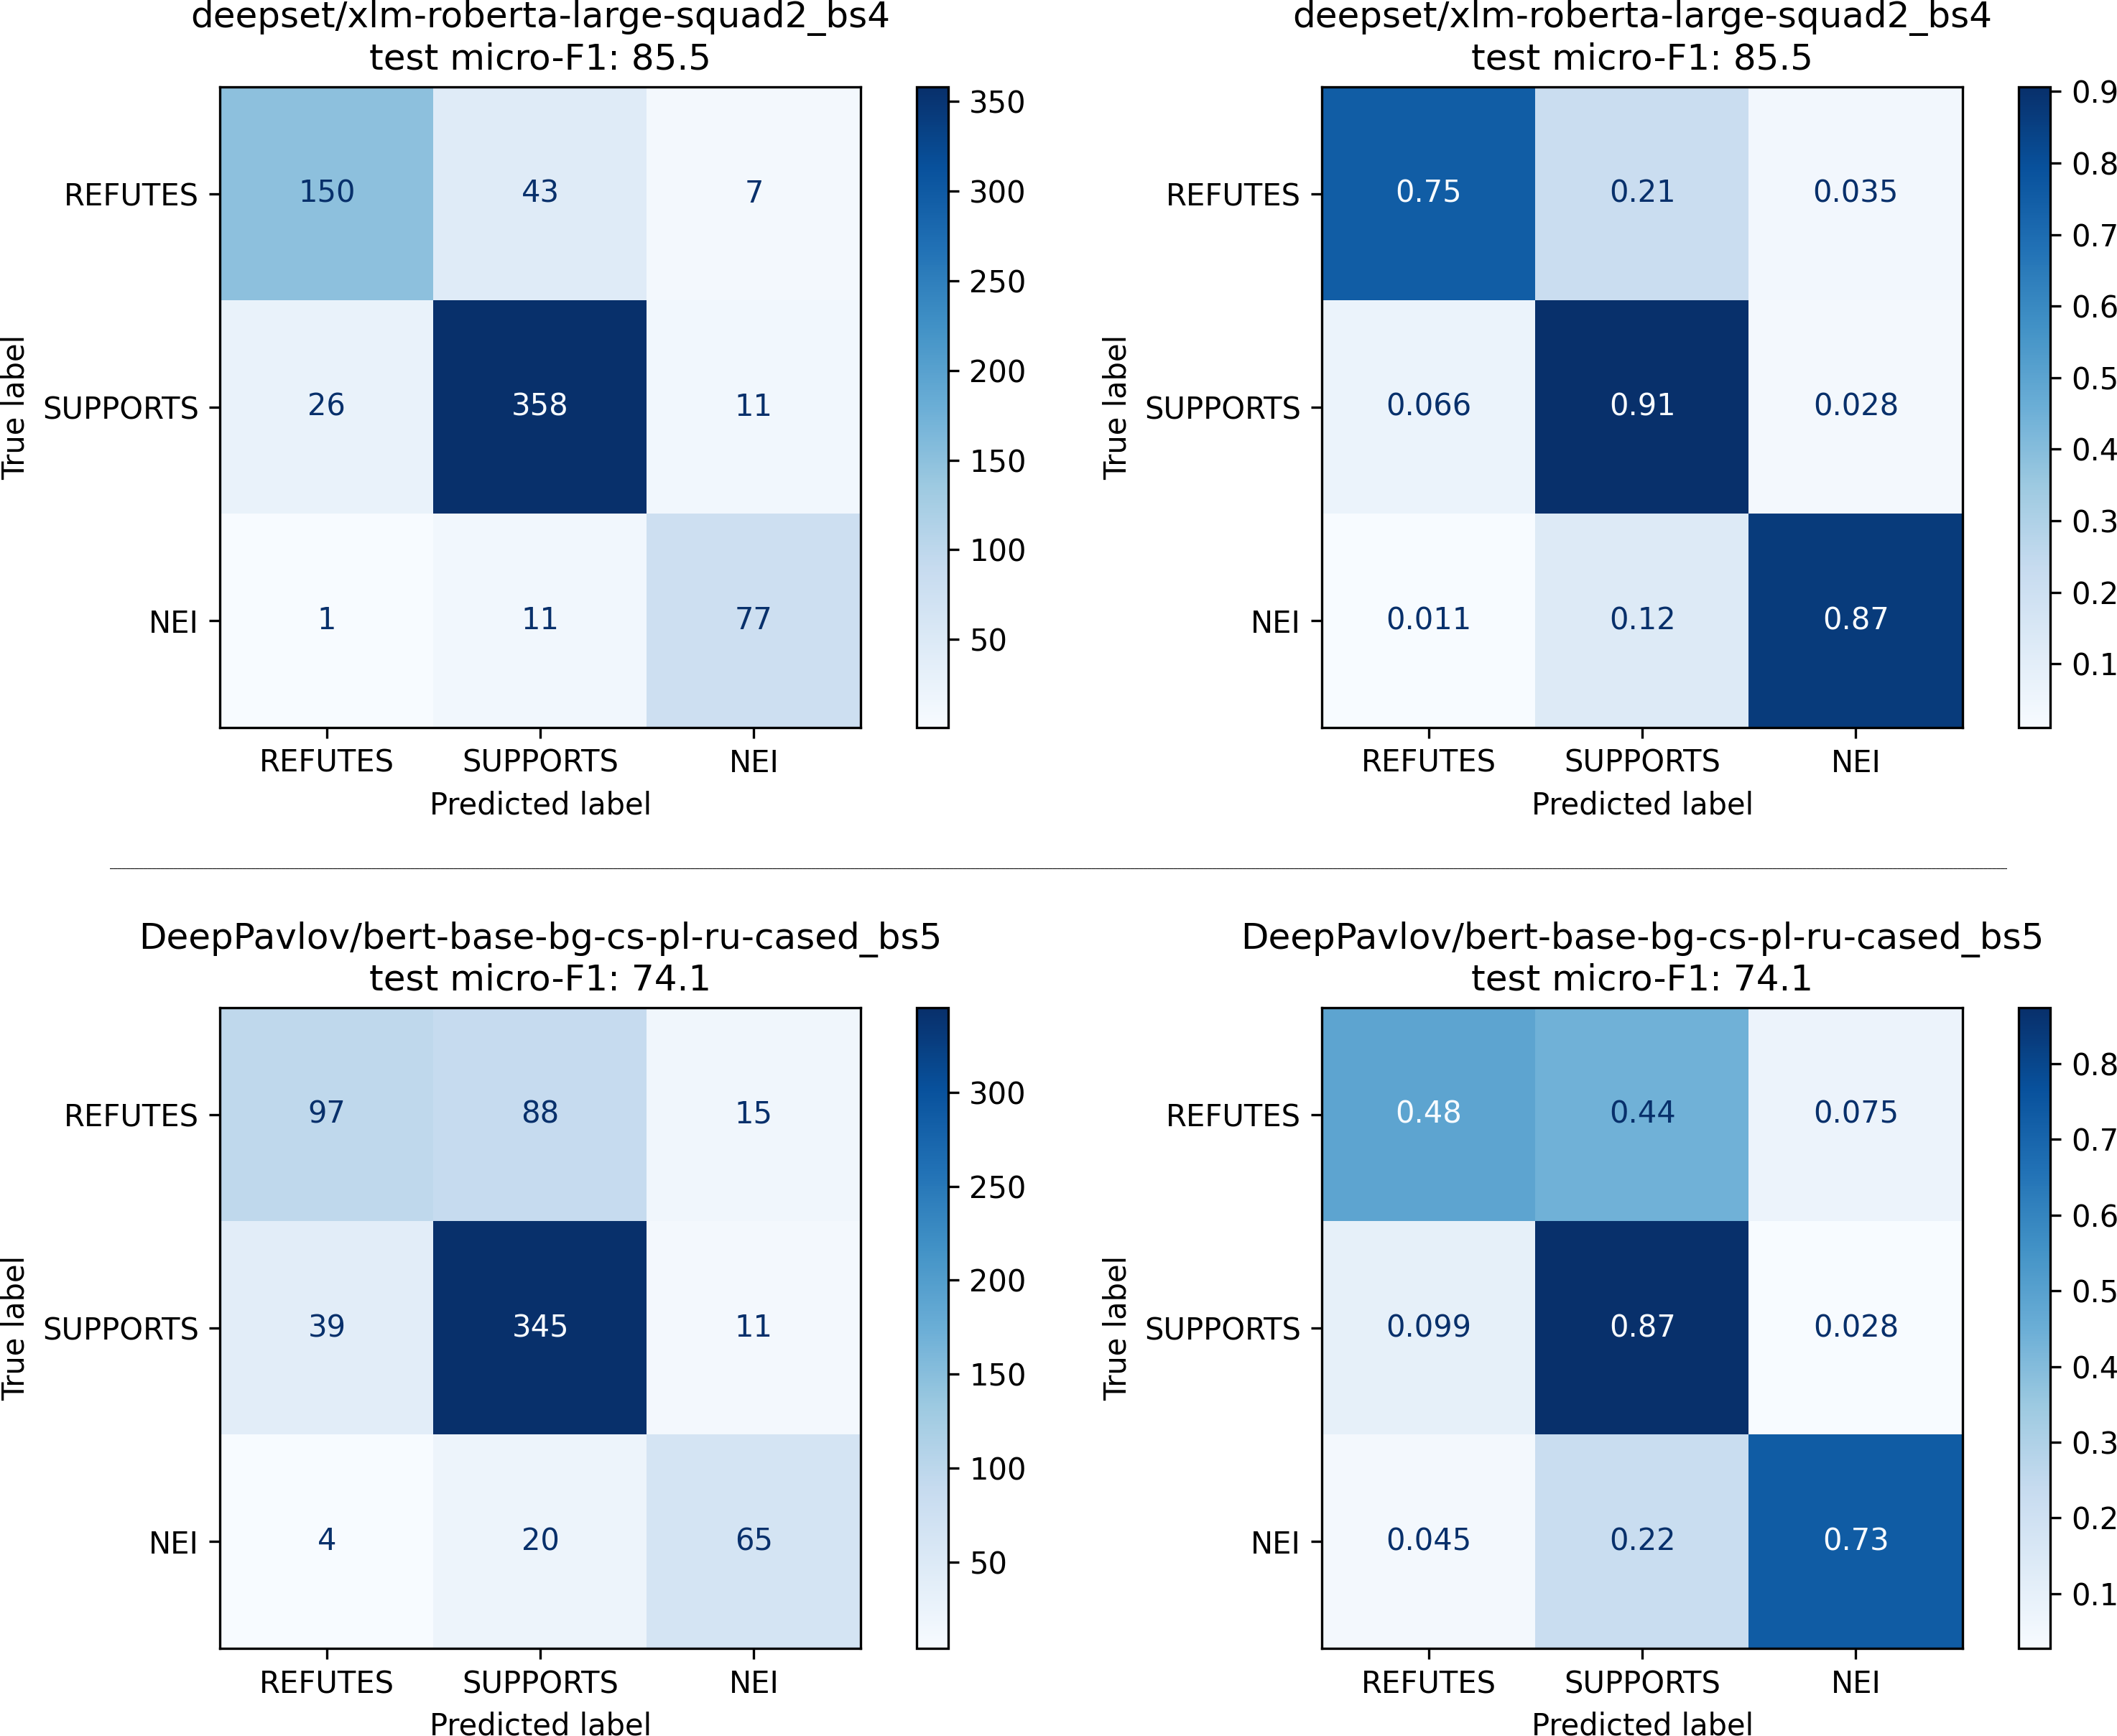
\includegraphics[width=17cm]{fig/confmat.png}}
\caption[Confusion Matrices of XLM-RoBERTa and SlavicBERT]{The confusion matrices of \textsf{XLM-RoBERTa} finetuned on \textit{SQuAD2} and the \textsf{SlavicBert} models for Natural Language Inference on \textsf{ČTK} test data}
\label{fig:confmat}
\end{figure} %confmatky
%--- /FIG



\subsection{Machine-translated NLI corpora}
To address the \textit{overfitting} (Table~\ref{tab:overfitting}) issue in our future experiments, our team at \textsf{AIC} has internally obtained a machine-translated Czech localization for each of the corpora listed in~\ref{sec:nlicorp},  using the \textsf{Google Translate API}. The scheme is simpler than that from~\ref{sec:fevercs}, as their formats are closely resemblant to the \texttt{nli} \textsf{FCheck} export (Figure~\ref{list:fcheck-nli}), i.e., a set of plain text pairs and their labels.

In future, the Czech \textsf{SNLI}, \textsf{MultiNLI}, \textsf{ANLI} or \textsf{FEVERNLI} datasets could be either used directly to augment the \textsf{ČTK NLI train} dataset, or to construct a \textit{down-stream task} for NLI in Czech.

In the weeks subsequent to the submission of this thesis, we will examine the licensing of the aforementioned corpora, and, if allowed, publish their Czech localizations in a cloud storage\footnote{\texttt{http://bertik.net/nli\_corpora}} to supplement this thesis.


\section{Experiments Wrapup}
In our last full chapter, we have used the data collected during our annotation experiments in Chapter~\ref{chap:ctk} to train a round of Czech Natural Language Inference classifiers. The strongest of them, \textsf{XLM-RoBERTa} sets a vital benchmark for its future successors, and is ready to be experimentally used in the production environment, provided there is a reliable \textit{Document Retriever} to feed its input (Figure~\ref{fig:pipeline}).

We attach the experimental notebooks\footnote{\url{https://gitlab.fel.cvut.cz/factchecking/nli}} used to train and validate our models, as well as the resulting model\footnote{\url{http://bertik.net/ctk-xlm-roberta}} in a hope for reproducibility of our experiments, however, the code quality is incomparable with the PHP application from Chapter~\ref{chap:ctk}.
